\documentclass{article}
\usepackage{amsmath}
\usepackage[T1]{fontenc}     % Needed for Polish words
\usepackage{graphicx}

\begin{document}

\title{Value Iteration and Q-Learning Algorithms}
\author{Kajetan Frąckowiak}
\date{26.03.2025}
\maketitle

\section{Value Iteration Algorithm}
Valute Iteration is a reinforcment learning method that updates state values iteratively using the Bellman equation:
\begin{equation}
    V^(s) = \max_a \sum_{s'} P(s'|s, a) \left[R(s, a, s') + \gamma V^(s')\right]
\end{equation}

where: \begin{itemize}
    \item $V^*(s)$ is the optimal value function. \item $P(s'|s, a)$ is the transition probability.
    \item $R(s, a, s')$ is the reward.
    \item $\gamma$ is the discount factor.
\end{itemize}

The algorithm iterates by computing action values and updating state values accordingly.

\section{Q-Learning Algorithm}
Q-Learning is a model-free reinforcment learning algorithm that updates the state-action value function using:
\begin{equation}
    Q(s, a) = Q(s, a) + \alpha \left[R(s, a, s') + \gamma \max_{a'} Q(s', a') - Q(s, a)\right]
\end{equation}

where: \begin{itemize}
    \item $Q(s, a)$ is the action-value function.
    \item $R(s, a, s')$ is the immediate reward.
    \item $\gamma$ is the discount factor.
    \item $max_{a'} Q(s', a')$ estimates future rewards.
\end{itemize}

The following chart presents the history of rewards obtained during training with Value Iteration and Q-Learning.

\begin{center}
    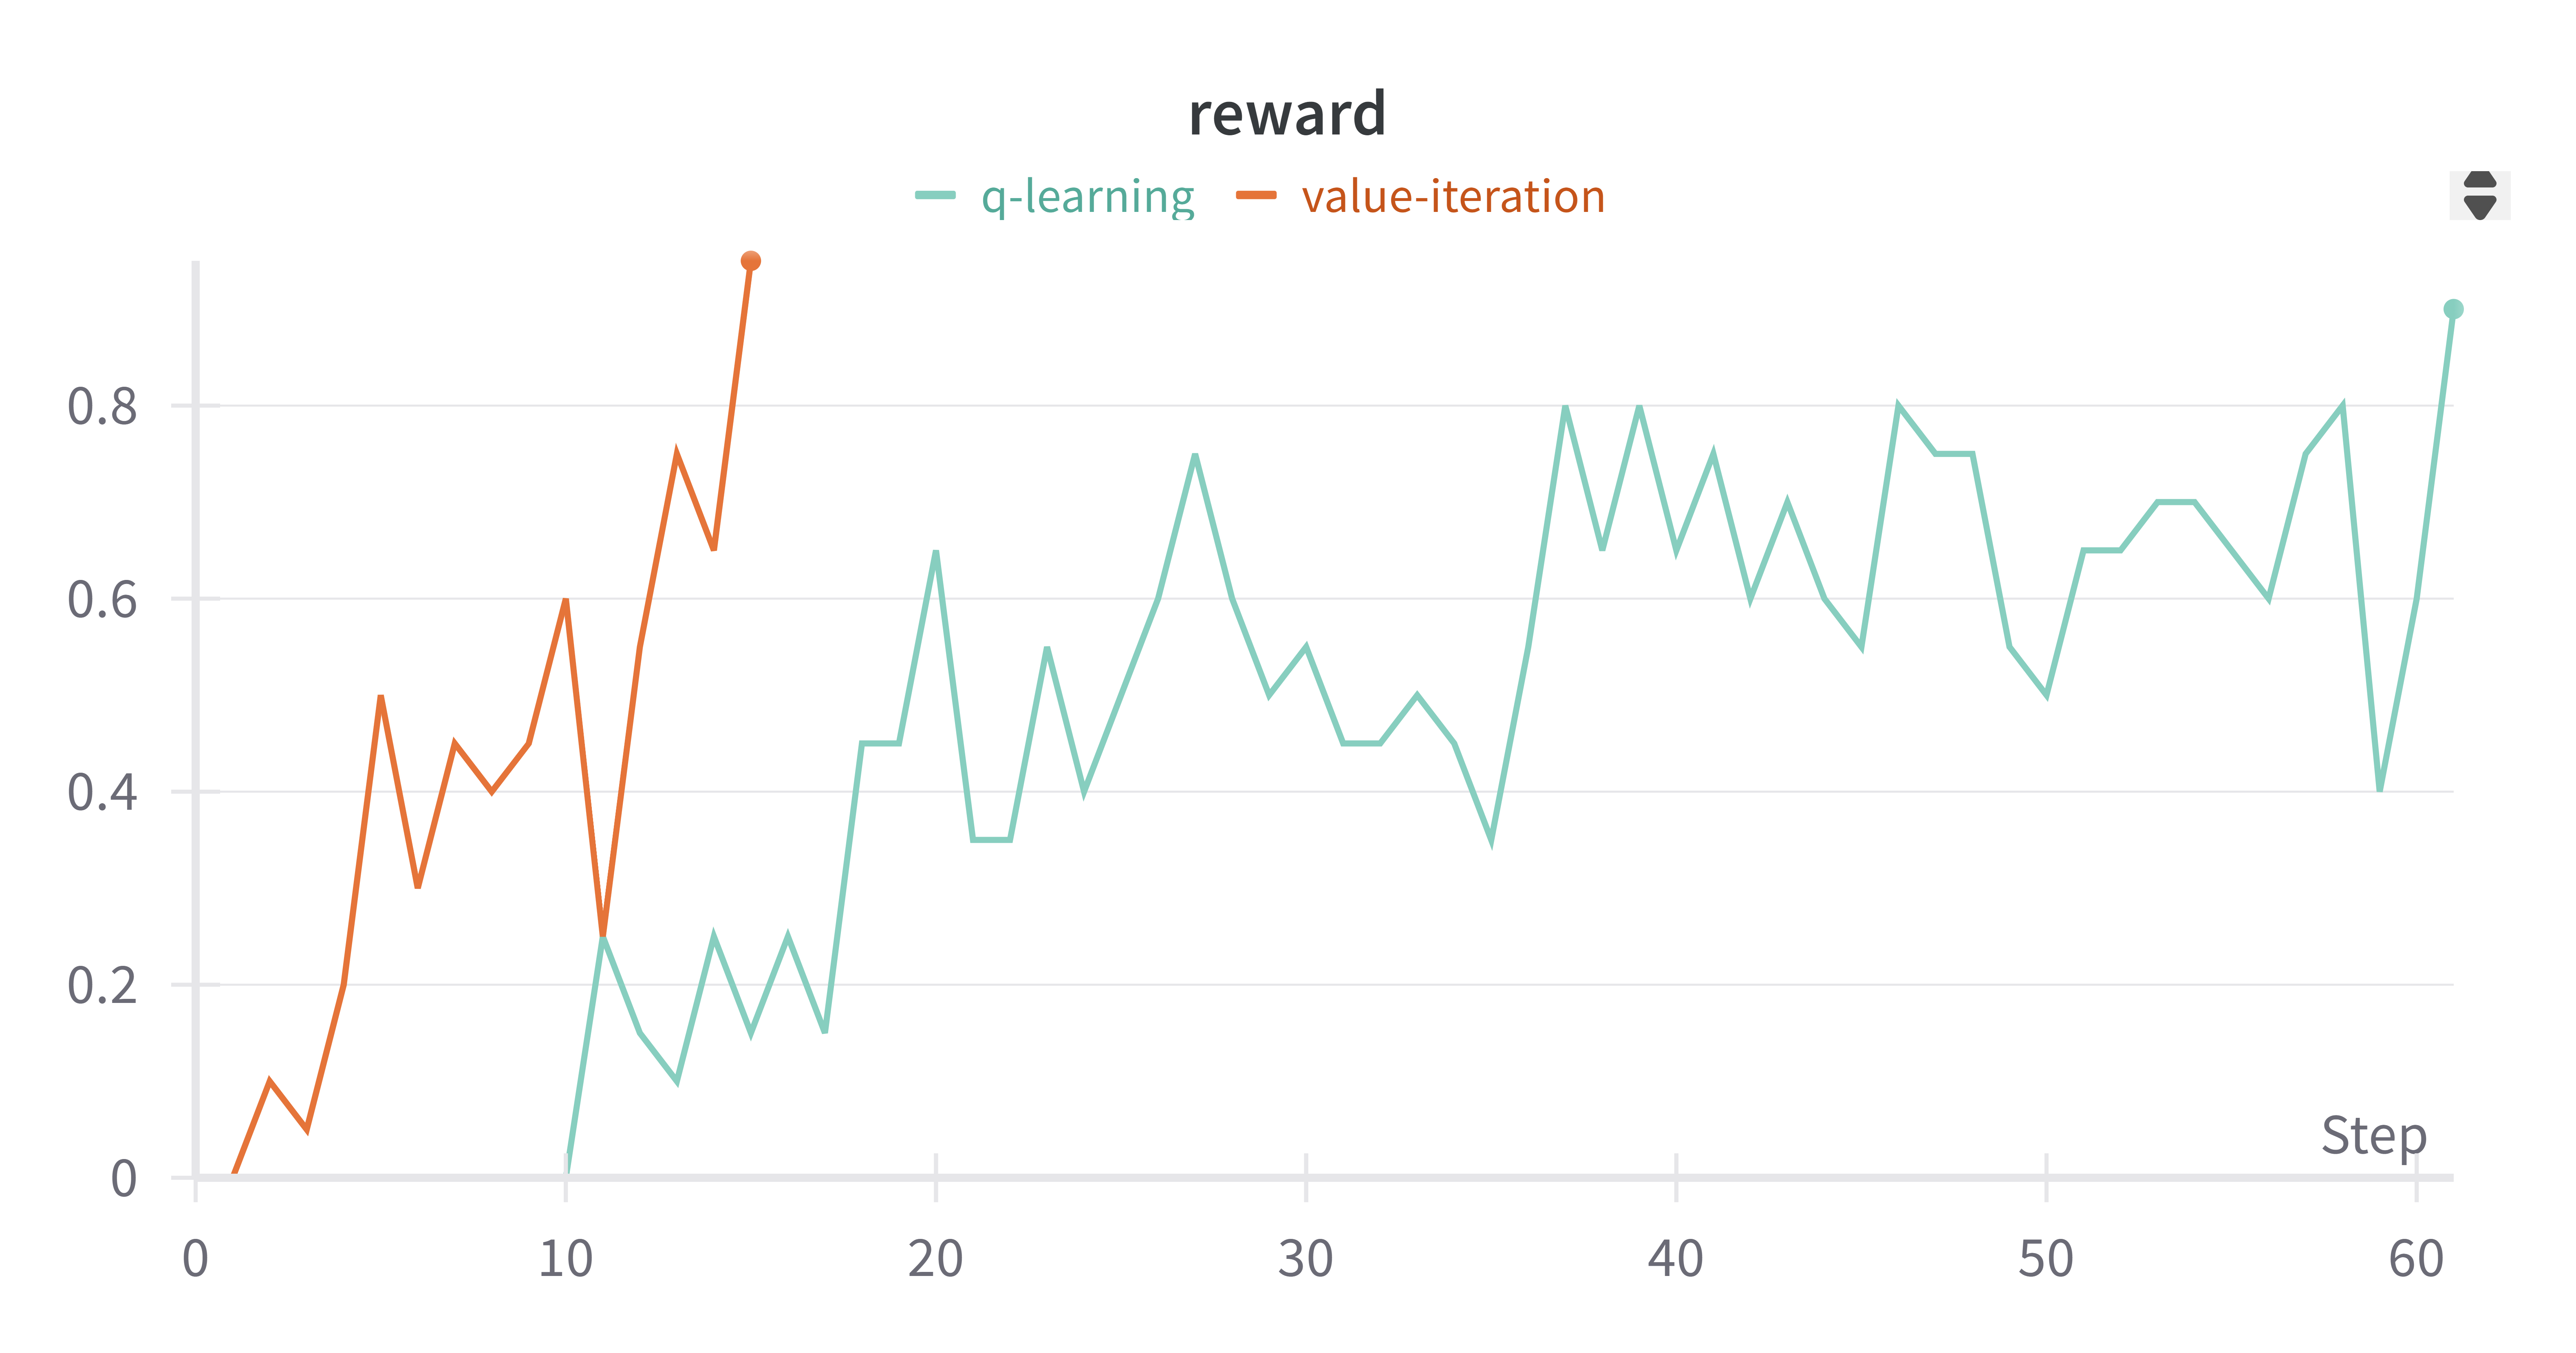
\includegraphics[width=0.8\textwidth]{reward.png}
\end{center}

\section{Summary}
As we can see, both Value Iteration like Q-Learning work well without gradient on FrozenLake-v1 with very few iterations. We plan to test it on other environments in future.

\end{document}